\documentclass{beamer}
%
% Choose how your presentation looks.
%
% For more themes, color themes and font themes, see:
% http://deic.uab.es/~iblanes/beamer_gallery/index_by_theme.html
%
\mode<presentation>
{
  \usetheme{default}      % or try Darmstadt, Madrid, Warsaw, ...
  \usecolortheme{default} % or try albatross, beaver, crane, ...
  \usefonttheme{default}  % or try serif, structurebold, ...
  \setbeamertemplate{navigation symbols}{}
  \setbeamertemplate{caption}[numbered]
} 

\usepackage[spanish]{babel}
\usepackage[utf8x]{inputenc}
\title[Clase 6]{Procesamiento de bases de datos con STATA}
\subtitle{Clase 6}
\author{Claudia Vazquez}
\date[]{\texttt{clauvazqu@gmail.com}\\Centro REDES}
\pgfdeclareimage[height=0.5cm]{university-logo}{logo-redes}
\logo{\pgfuseimage{university-logo}}

\begin{document}

\begin{frame}
  \titlepage
\end{frame}

\begin{frame}
\tableofcontents
\end{frame}

\begin{frame}{Introducción}
\begin{itemize}
\item En esta clase aprenderemos a realizar test de hipótesis y estimar modelos en STATA.
\item No nos extendemos en las características de los modelos y test sino en su implementación en STATA.
\item Para un mayor detalle sobre los modelos econométricos se recomienda:
\begin{itemize}
\item Wooldridge, J. M. (2001), \textit{Introducción a la econometría. Un enfoque moderno}. Thomson Learning. Mexico.	
\item Davidson, R. y MacKinnon, J., (2004), \textit{Econometric Theory and Methods}, Oxford.
\item Kmenta, J (1977), \textit{Elementos de Econometría}. Vicens Vives. Barcelona. 
\end{itemize}
\end{itemize}
\end{frame}

\section{Test de comparación de medias}

\begin{frame}{Two sample t-test}{Introducción}
\begin{itemize}
\item Muchas veces queremos comparar el valor de alguna variable entre dos grupos. Por ejemplo: 
\begin{itemize}
\item ?`Los hombres tienen, en promedio, mayores salarios que las mujeres? 
\item ?`Los pacientes que recibieron la nueva medicacion durante un ensayo clínico tienen, en promedio, menos colesterol que los pacientes que recibieron placebo?
\end{itemize}
\item Lo que nos interesa es saber si las medias son \textbf{estadísticamente} diferentes.
\item Podemos relizar un test de comparación de medias entre dos grupos o \textit{t-Test}.
\end{itemize}
\end{frame}
\subsection{test a dos colas}
\begin{frame}[allowframebreaks]{Two sample t-test}{test a dos colas}
\begin{itemize}
\item La hipótesis nula en un test a dos colas es que las medias de ambos grupos son iguales. La hipótesis alternativa, que son distintas: 
\begin{displaymath}
\left\{ \begin{array}{l}
H_{0}: \mu_{1} = \mu_{2} \\ 
H_{1}: \mu_{1} \neq  \mu_{2} 
\end{array} \right.
\end{displaymath}
\item Ejemplo: queremos probar la eficacia de un nuevo aditivo para el combustible. Cargamos una base de datos con información para 24 autos, 12 con el aditivo y 12 sin:\\
\small{\texttt{use http://www.stata-press.com/data/r12/fuel3}}
\item La variable continua sobre la que queremos evaluar la diferencia es ``mpg''.
\item La variable categórica que forma los grupos es ``treated'', que vale 1 si el auto recibió el tratamiento y 0 en otro caso. 
\begin{center}
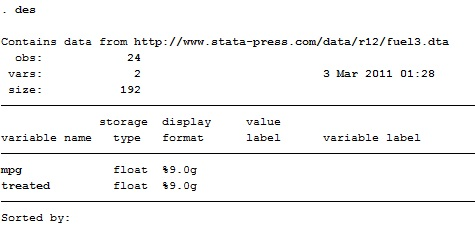
\includegraphics[height=4.5cm]{ttest0.jpg}
\end{center}
\item A continuación realizamos el t-Test para ver si la diferencia de medias entre los dos grupos es significativa:
\end{itemize}
\begin{center}
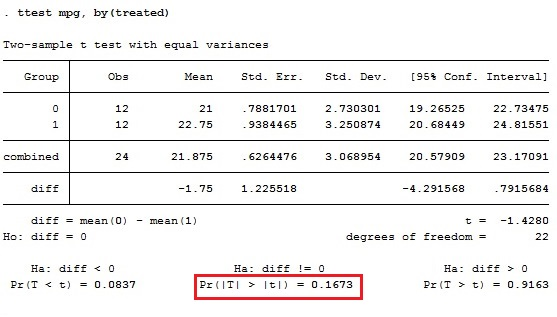
\includegraphics[height=4.5cm]{ttest1.jpg}
\end{center}
\begin{itemize}
\item Como el \textit{p-value} de 0.1673 es mayor que 0.05, no podemos rechazar $H_{0}$ y concluimos que las medias no son estadísticamente distintas.
\end{itemize}
\begin{itemize}
\item En el ejemplo anterior, se asumía que los dos grupos tenían la misma varianza. 
\item Si no estamos dispuestos a asumir esto, agregamos la opción \texttt{welch} en el comando \texttt{ttest}: \\
\begin{center}
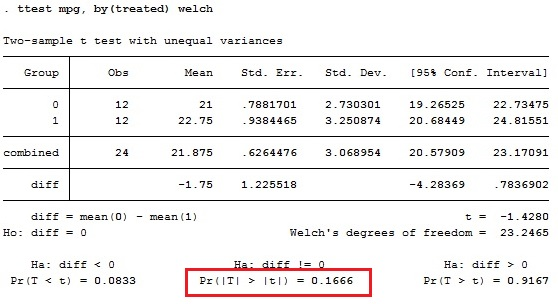
\includegraphics[height=4.5cm]{ttest2.jpg}
\end{center}
\item En este caso tampoco tenemos evidencia suficiente para rechazar $H_{0}$.
\end{itemize}
\end{frame}
\subsection{test a una cola}
\begin{frame}[allowframebreaks]{Two sample t-test}{test a una cola}
\begin{itemize}
\item En muchas situaciones podemos estar interesados en alguna dirección particular de la desigualdad en las medias. 
\item Por ejemplo, podemos pensar que la media de la población 1 es mayor que la media de la población 2.
\item En ese caso, realizamos el test a una cola:\\
\begin{displaymath}
\left\{ \begin{array}{l}
H_{0}: \mu_{1} \leq \mu_{2} \\ 
H_{1}: \mu_{1} > \mu_{2} 
\end{array} \right.
\end{displaymath}
\item La región crítica del test de hipótesis se ubica a la derecha.\\\smallskip
\begin{center}
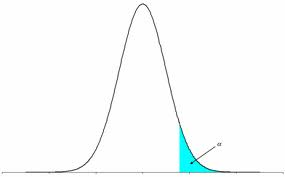
\includegraphics[height=2cm]{ttest3.jpg}
\end{center}
\item La ventaja del test a una cola es que aumenta la potencia: si estábamos en lo correcto respecto de la dirección de la diferencia, es más probable que detectemos una diferencia significativa con un test a una cola que con uno a dos.
\item La sintaxis para implementar el test a una cola en STATA es la misma, simplemente miramos otro \textit{p-value}:\\
\begin{center}
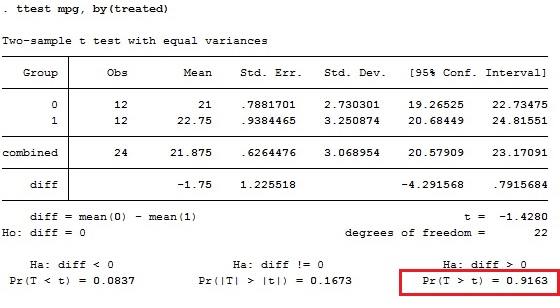
\includegraphics[height=4.5cm]{ttest4.jpg}
\end{center}
\end{itemize}
\end{frame}


\section{Análisis de Varianza (ANOVA)}

\subsection{One way ANOVA}

\begin{frame}[allowframebreaks]{One way ANOVA}
\begin{itemize}
\item Si queremos testear hipótesis sobre la diferencia de medias en más de dos grupos podemos usar ANOVA.
\item Supongamos que tenemos una variable dependiente continua y una variable independiente categórica con muchos niveles, no solo dos.
\item ANOVA nos ayuda a determinar si las diferencias en las medias son lo suficientemente grandes como para indicar que las medias poblacionales son distintas. 
\item La hipótesis nula es: \\
\begin{center}
$H_{0}: \mu_{1} =  \mu_{2} = \mu_{3} = \mu_{4}$
\end{center}
\item La hipótesis alternativa es que no todas las medias poblacionales son iguales: al menos una es diferente.
\item Como ejemplo, analizamos la efectividad de cuatro fertilizantes distintos en el peso de las manzanas. 
\item La información del fertilizante utilizado y el peso en gramos está en la siguiente base de datos: \small{\texttt{http://www.stata-press.com/data/r12/apple}}
\item Nuestro modelo explica la variabilidad en el peso de la fruta a partir del fertilizante utilizado: \\
\begin{center}
$Y_{ij}= \mu + \tau_{j} + \epsilon_{ij}$
\end{center}
\item $i$ representa a la observación e $j$, al tipo de fertilizante. 
\item $\mu$ es el peso promedio de la fruta en toda la muestra, independientemente del fertilizante. 
\item $\tau_{j}$ es el efecto de cada uno de los fertilizantes: por ejemplo $\tau_{1}$ es la diferencia en el peso promedio con el fertilizante 1, etc.
\item $\epsilon_{ij}$ es el término de error, también conocido como la variabilidad \textit{within} o no explicada: representa la variación en el peso de la fruta que no está explicada por el uso de diferentes tipos de fertilizantes.
\item ANOVA analiza la varianza de los datos para determinar si existe una diferencia en la media de los distintos grupos. \\
\begin{center}
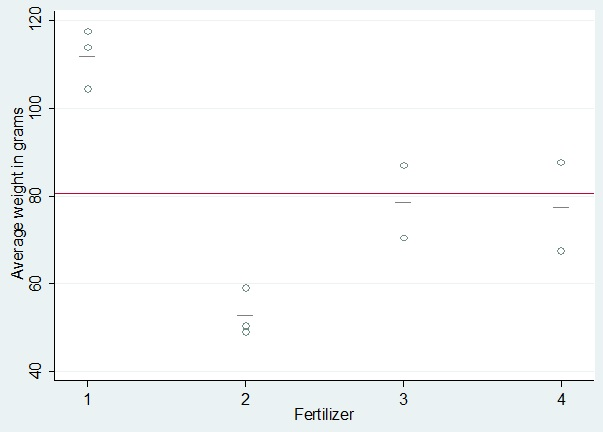
\includegraphics[height=5.4cm]{oneway1.jpg}
\end{center}
\begin{center}
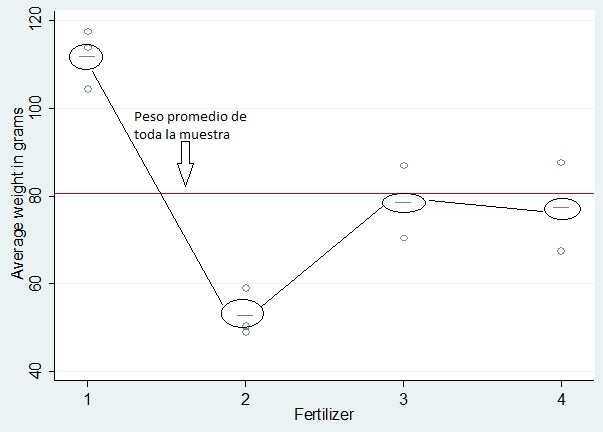
\includegraphics[height=5.2cm]{oneway1a.jpg}\\\medskip
Variabilidad de las medias entre los grupos (``\textit{Between-Group}'')
\end{center}
\begin{center}
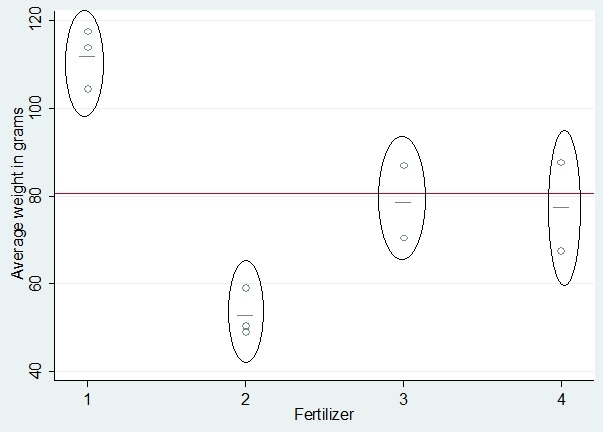
\includegraphics[height=5.2cm]{oneway1b.jpg}\\\medskip
Variación de los datos al interior de los grupos (``\textit{Within-Group}'')
\end{center}
\item Si la variabiliad ``between'' es significativamente superior a la variabilidad ``within'', rechazamos la hipótesis nula de que las medias de todos los grupos son iguales.
\item Para particionar la variabiliad usamos la suma de cuadrados: \\
\begin{displaymath}
\underbrace{\sum n_{i}(\overline{Y_{i}}-\overline{\overline{Y}})^2}_{SSM} + \underbrace{\sum \sum (Y_{ij}-\overline{Y_{i}})^2}_{SSE} = \underbrace{\sum \sum (Y_{ij}-\overline{\overline{Y}})^2}_{SST}
\end{displaymath}
\item El primer término (\textit{Model Sum of Squares}) corresponde a la variabilidad ``between''.
\item El segundo (\textit{Error Sum of Squares}) corresponde a la variabilidad ``within''.
\item El último (\textit{Total Sum of Squares}) es la suma total.
\item Para implementar one way ANOVA en STATA utilizamos el comando \texttt{oneway}:\\
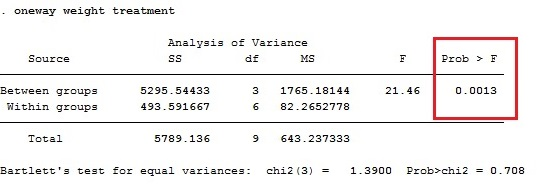
\includegraphics[height=3.5cm]{oneway2.jpg}
\item El \textit{p-value} es menor a 0.05 por lo que rechazamos la hipótesis de que las medias sean iguales: existen diferencias significativas en el peso de la fruta entre los diferentes fertilizantes.
\end{itemize}
\end{frame}

\subsection{Two-way ANOVA}

\begin{frame}[allowframebreaks]{Two-way ANOVA}
\begin{itemize}
\item Cuando queremos ver el efecto de dos o más variables categóricas usamos two-way ANOVA (o \textit{n}-way ANOVA).
\item En ese  caso, además del efecto de cada una sobre la variable dependiente, podemos querer ver si existen interacciones entre ellas.
\item El modelo incluye el efecto de los diferentes niveles de la variable $\alpha$; los de la variable $\beta$ y de las posibles combinaciones entre ambas ($\alpha\beta$):
\begin{displaymath}
Y_{ijk}= \mu + \alpha_{i} + \beta_{j} + (\alpha\beta)_{ij} + \epsilon_{ijk}
\end{displaymath}
\item Como ejemplo utilizamos una base de datos con información sobre 58 pacientes.\\
\footnotesize{\texttt{use http://www.stata-press.com/data/r12/systolic}}\\
\item Los pacientes tenían alguna de las tres enfermedades estudiadas y fueron asignados aleatoriamente a alguno de los cuatro tratamientos, que consistieron en suministrar diferentes dosis de un medicamento. 
\item Después del tratamiento se midieron los cambios en la presión sanguínea.  
\begin{center}
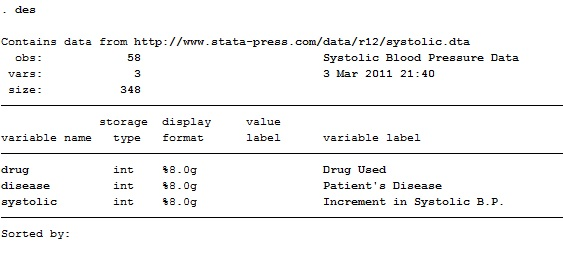
\includegraphics[height=4cm]{twoway.jpg}
\end{center}
\item Queremos ver si el tratamiento y la enfermedad previa afectan la presión sanguínea. Además, queremos ver si la enfermedad y el tratamiento interactúan en el efecto sobre la variable dependiente (ej. el efecto del tratamiento depende de qué enfermedad presente el paciente).
\begin{center}
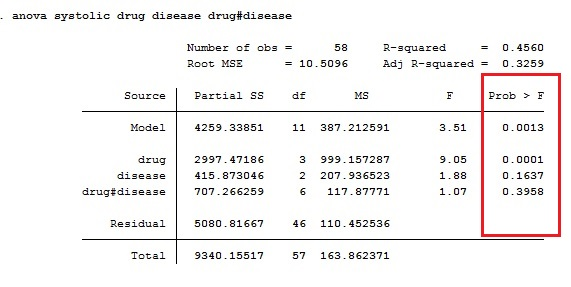
\includegraphics[height=5cm]{twoway1.jpg}
\end{center}
\item En el análisis de ANOVA vemos que el único factor que resulta significativo es el tratamiento (variable ``drug'').
\end{itemize}
\end{frame}



\section{Modelo de regresión lineal}
\subsection{Análisis exploratorio de los datos}
\begin{frame}[allowframebreaks]{Análisis exploratorio de los datos}
\begin{itemize}
\item Es importante conocer los datos antes de estimar modelos.
\item Siempre realizamos un análisis exploratorio, que puede incluir: 
\begin{itemize}
\item Gráficos (scatter plot)
\item Análisis de correlación
\end{itemize}
\item Los gráficos pueden ayudarnos a identificar \textit{outliers} y tendencias en los datos.
\item Cargamos la base auto.dta.
\item Queremos conocer la relación entre las variables continuas ``mpg'' y ``weight''. \\\bigskip
\texttt{twoway scatter mpg weight}
\begin{center}
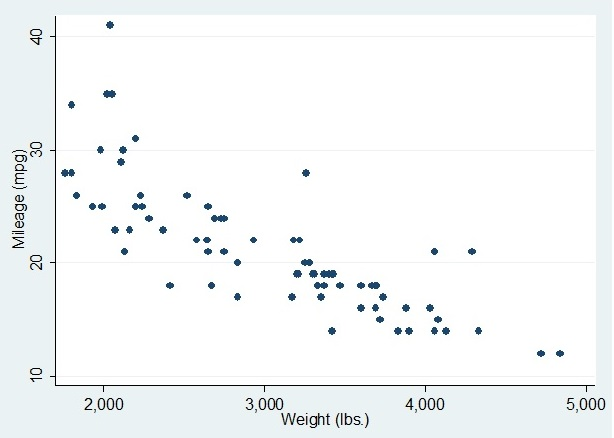
\includegraphics[height=4.5cm]{scatter.jpg}
\end{center}
\item Con el comando \texttt{correl} podemos medir la correlación lineal entre las variables. 
\item Las variables pueden tener una asociación lineal positiva, negativa o pueden no estar asociadas linealmente. \\\smallskip
\begin{center}
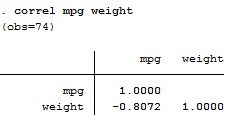
\includegraphics[height=2.7cm]{correl.jpg}
\end{center}
\item El coeficiente de correlación de Pearson varía entre 1 y -1.
\item Hay que se muy cautelosos con la interpretación: correlación no implica causalidad.
\item Una correlación muy fuerte entre dos varibles puede deberse a: 
\begin{itemize}
\item Alguna de las dos variables es causa de la otra.
\item Existe/n otra/s variable/s que afecta/n a ambas.
\item Casualidad.
\end{itemize}
\end{itemize}
\end{frame}
\subsection{El modelo lineal}
\begin{frame}{El modelo lineal}
\begin{itemize}
\item Suponemos que $y$ (variable dependiente) y $x$ (variable independiente) se encuentran relacionadas de la siguiente forma: 
\end{itemize}
\begin{equation}
y_{i}=\beta_1 + \beta_2 x_{i} + u_{i}
\end{equation}
\begin{itemize}
\item Donde $\beta_1$ y $\beta_2$ son coeficientes desconocidos y $u_i$ es una variable aleatoria no observada que representa el hecho de que la relación entre $x$ e $y$ no es exacta.
\item El comando \texttt{regress} estima este modelo por MCO. La sintaxis consiste en indicar primero la variable dependiente y luego la/s variable/s independiente/s.
\end{itemize}
\end{frame}

\begin{frame}{Ejemplo modelo lineal}
\begin{itemize}
\item Usamos la base ``muestra.dta'' con información socio laboral para 1.204 individuos. 
\item Estimamos un modelo donde la variable dependiente es el logaritmo del salario y las variables independientes los años de educación y la experiencia laboral:\\\smallskip
{\footnotesize \texttt{regress lwage educ exper}}
\end{itemize}
\centerline{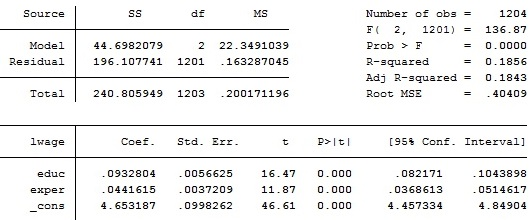
\includegraphics[height=3.2cm]{reg.jpg}}
\end{frame}

\begin{frame}{Output}
\begin{itemize}
\item Arriba a la izquierda se presenta un análisis de la varianza (ANOVA): la varianza total se descompone en la explicada por el modelo y la residual.
\item Arriba a la derecha se presenta:
\begin{itemize} 
\item el estadístico $F$ asociado a la tabla ANOVA, que contrasta la hipótesis de que todos los coeficientes excluída la constante son cero (\textit{test} de significatividad global).
\item el \textit{p-value} asociado al test de significatividad global.
\item el $R^{2}$ y el $R^{2}$ ajustado.
\item el desvío estándar del término de error (MSE).
\end{itemize}
\item Luego se presenta la tabla de coeficientes con:
\begin{itemize}
\item valor y desvío estándar del coeficiente estimado.
\item estadístico $t$ y el \textit{p-value} que indica el nivel de significatividad (dos colas).
\item intervalo de confianza para el coeficiente estimado.
\end{itemize}
\end{itemize}
\end{frame}

\begin{frame}{Variables independientes categóricas}
\begin{itemize}
\item En la base tenemos una variable categórica (``región'') que toma valores 1, 2 y 3 según la región donde vive el individuo. 
\item Para controlar por esta variable incluimos en el modelo dos variables \textit{dummy}: 
\begin{itemize}
\item Una que vale 1 cuando región=2 y 0 en otro caso.
\item Otra que vale 1 cuando región=3 y 0 en otro caso. 
\end{itemize}
\item ``región=1'' es la categoría base, por lo que los coeficientes que acompañan a las otras dos variables miden el cambio respecto a este grupo.
\item Las  \textit{dummy} se pueden crear previamente o indicarle a STATA que lo haga escribiendo ``i.'' antes del nombre de la variable.
\end{itemize}
\end{frame}

\begin{frame}{Variables independietes categóricas}{}
{\footnotesize \texttt{regress lwage educ exper i.region}}\\\medskip
\centerline{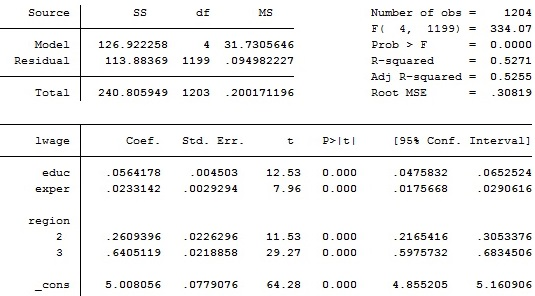
\includegraphics[height=4.2cm]{reg2.jpg}}
\end{frame}

\section{Regresión logística}

\begin{frame}{Variables dependientes dicotómicas}
\begin{itemize}
\item Cuando la variable dependiente es una variable dicotómica, el modelo lineal puede no ser la mejor opción, ya que los valores que predice para la variable dependiente pueden estar por fuera del intervalo [0, 1]. 
\item En estos casos, podemos utilizar el comando \texttt{logit}, que modela la probabilidad de que la variable dependiente sea igual a 1 (``positivo''), dado un conjunto de regresores. 
\item Por ejemplo, en la base tenemos una variable dicotómica llamada ``ingreso'' que vale 1 cuando el salario horario es mayor a 550 y cero cuando es menor.
\item Estimamos un modelo para la probabilidad de que el salario sea mayor a 550 dado el nivel de educación, la experiencia laboral y la región.
\end{itemize}
\end{frame}

\begin{frame}{Variables dependientes dicotómicas}{}
{\footnotesize \texttt{logit ingreso educ exper i.region}}\\\smallskip
\centerline{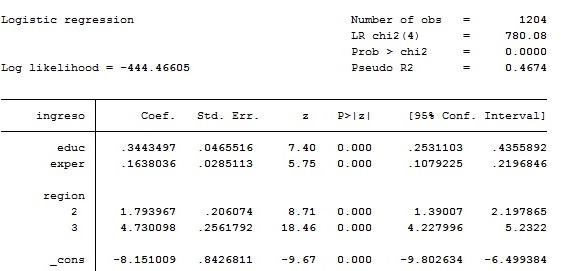
\includegraphics[height=3cm]{reg3.jpg}}
\begin{itemize}
\item Si bien la significatividad y el signo de los coeficientes tienen una interpretación similar al modelo lineal, el valor no es directamente interpretable ya que el efecto marginal no es constante sino que depende del punto donde se lo evalúe.
\end{itemize}
\end{frame}

\section{Algunos comandos post-estimación}
\subsection{predict y test}
\begin{frame}{Comandos post estimación}
\begin{itemize}
\item Después de realizar una estimación  podemos:
\begin{itemize}
\item usar el comando \texttt{test} para realizar test de hipótesis sobre los coeficientes. 
\item usar el comando \texttt{predict} para obtener los valores estimados y los residuos de la regresión.
\end{itemize}
\end{itemize}
{\footnotesize Ejemplo:}\\
{\footnotesize \texttt{regress  lwage educ exper exper2}}\\
{\footnotesize \texttt{predict ln\_sal\_e}}\\
{\footnotesize *crea una variable ``ln\_sal\_e'' con los valores estimados por el modelo}\\
{\footnotesize \texttt{predict errores, resid}}\\
{\footnotesize *crea una nueva variable llamada ``errores'' con los residuos del modelo}\\
{\footnotesize \texttt{test educ=0}}\\
{\footnotesize * testea la hipótesis de que el coeficiente que acompaña ``educ'' es 0}\\\medskip
\end{frame}
\subsection{outreg2}
\begin{frame}{Guardar y exportar los resultados}
\begin{itemize}
\item STATA ofrece opciones para guardar y ver los resultados de la estimación de distintos modelos.
\item En primer lugar deben instalar el siguiente comando escribiendo: \\
{\footnotesize \texttt{ssc install outreg2}}
\item Ahora podemos guardar los resultados de la siguiente manera: \\
{\footnotesize \texttt{regress lwage educ exper}}\\
{\footnotesize \texttt{estimates store Modelo1}}\\
{\footnotesize \texttt{regress lwage educ exper i.region}}\\
{\footnotesize \texttt{estimates store Modelo2}}
\item Para exportar los resultados al archivo excel ``resultados'':
\end{itemize}
{\footnotesize \texttt{outreg2 [Modelo1 Modelo2] using resultados.xls, replace}}

\end{frame}

\begin{frame}{Guardar y exportar los resultados}{archivo resultados.xls}
\centerline{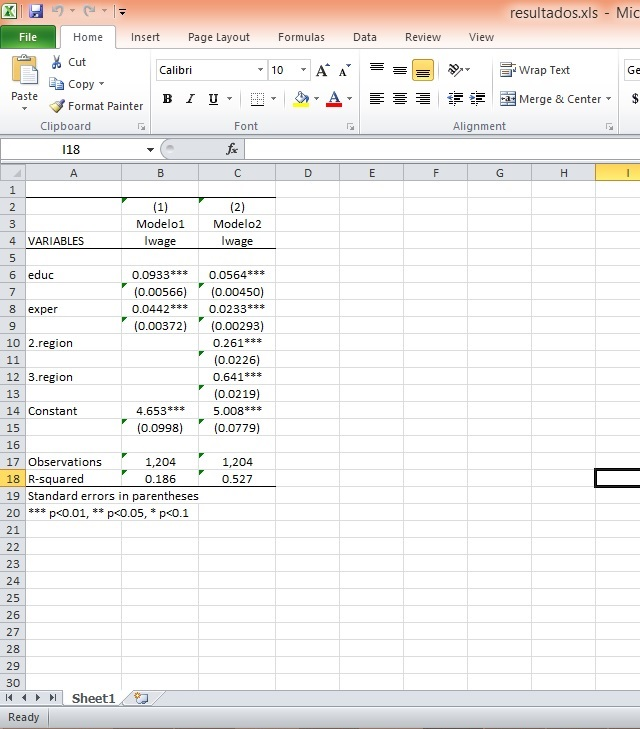
\includegraphics[height=7.5cm]{out.jpg}}
\end{frame}

\end{document}


\begin{frame}{Interpretación de los coeficientes}
\begin{itemize}
\item Los coeficientes estimados $\beta_k$ son la derivada \textbf{parcial} de la función de regresión respecto de la variable explicativa ($\x_k$). Suponen un \underline{efecto marginal} constante.
\item En el caso de las variables dicotómicas, el coeficiente estimado $\beta_k$ la diferencia constante entre el valor esperado cuando la variable vale 1 y el valor esperado de $y$ dado el vector $X$ cuando la variable $\x_k$ vale cero.
\end{itemize}
\end{frame}

\begin{frame}{Interacciones}

\end{frame}

\begin{frame}{Datos observacionales vs experimentos controlados}
\begin{itemize}
\item Queremos realizar inferencias sobre el efecto de una variable (tratamiento) pero la asignación de dicho tratamiento está fuera de nuestro control.  
\item Si en un experimento controlado el tratamiento se asigna de manera aleatoria, se reduce el efecto de los factores que afectan al fenómeno y están fuera de nuestro control
\item Variables de control: afectan a la variable de interés pero no :
\begin{displaymath}
Y_{ijk}=\mu + \alpha_{i} + \tau_{j} + \epsilon_{ijk}
\end{displaymath}
\end{itemize}
\end{frame}